\documentclass[tikz,border=6pt]{standalone}
\usepackage{amsmath}
\usetikzlibrary{arrows.meta,positioning,fit,backgrounds,calc}

\begin{document}
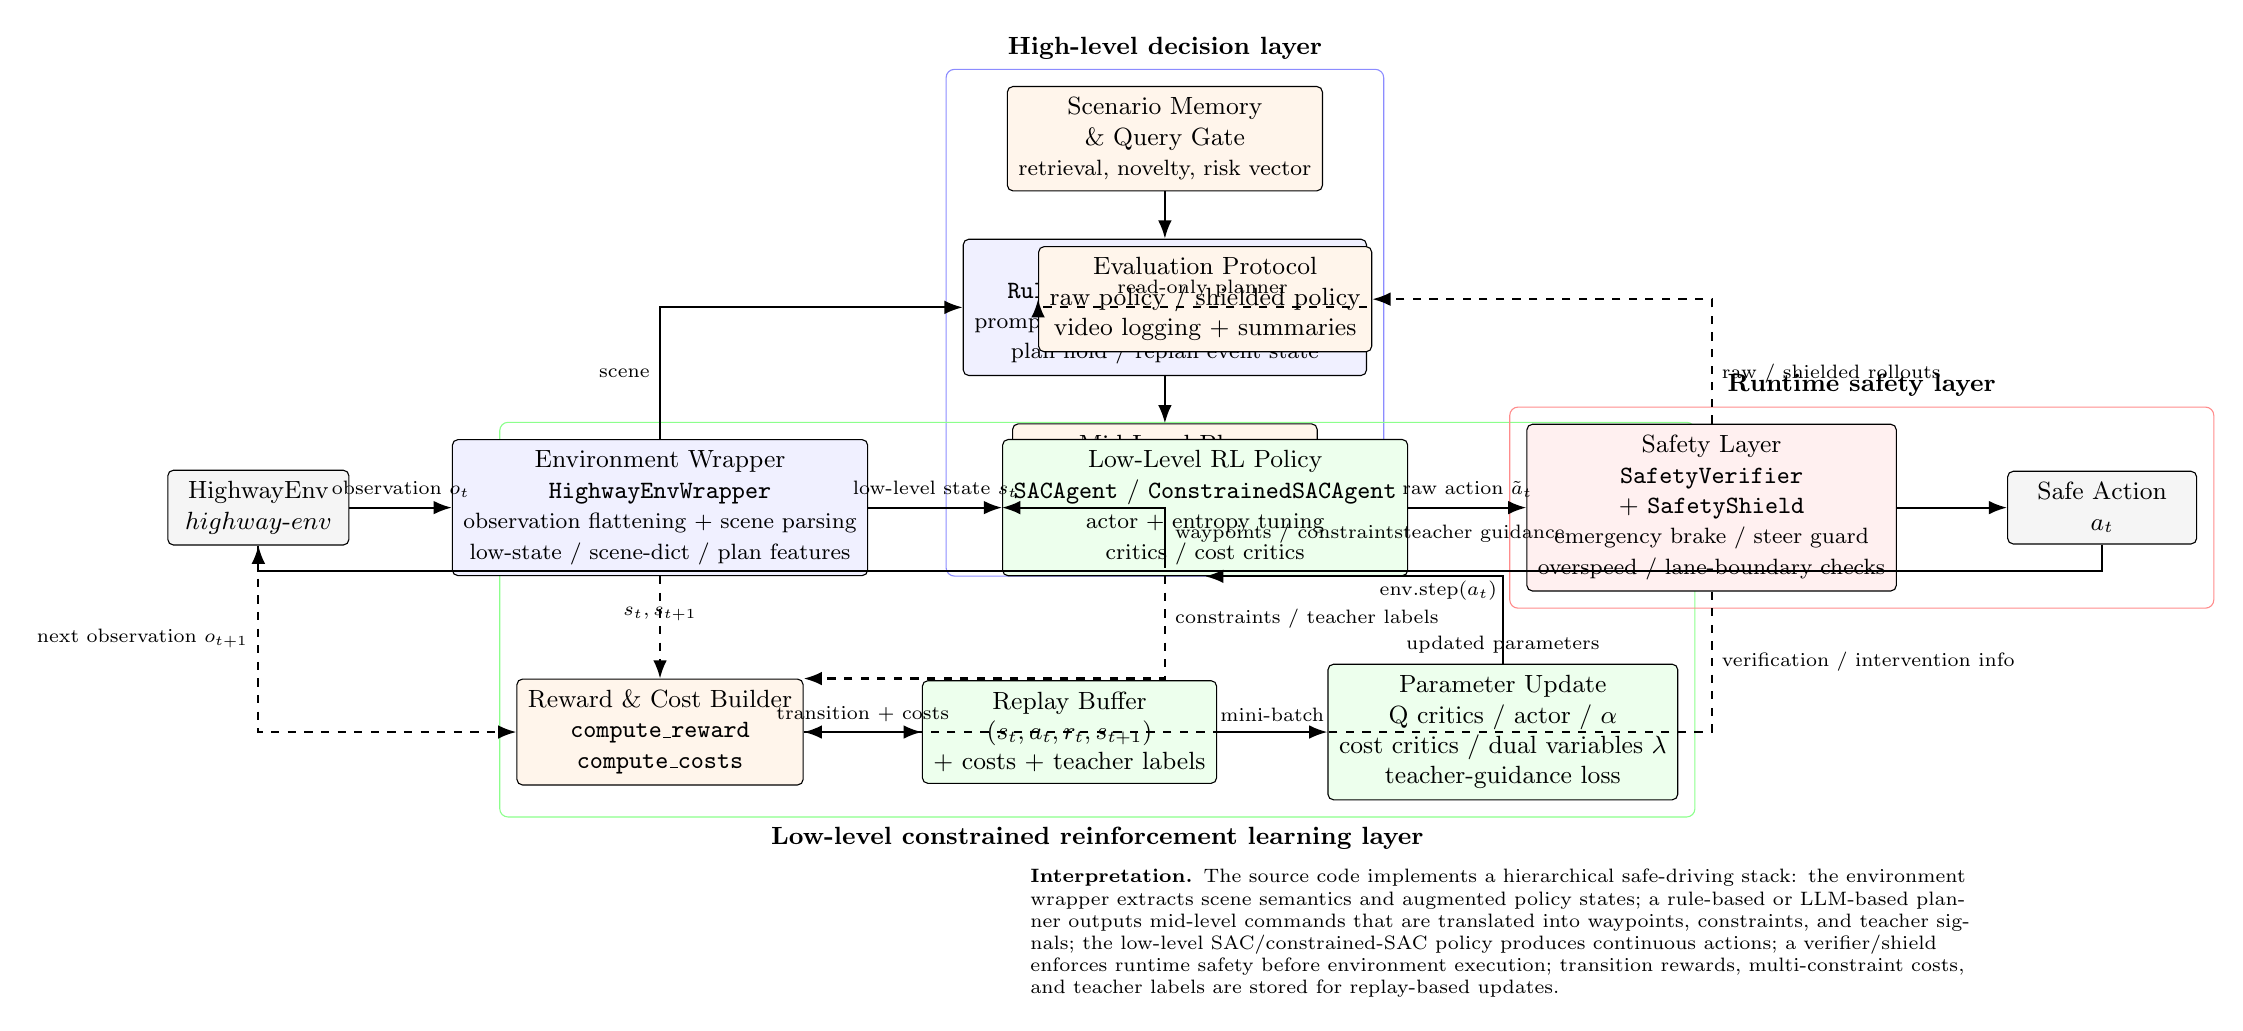
\begin{tikzpicture}[
    font=\small,
    >=Latex,
    node distance=7mm and 8mm,
    box/.style={draw, rounded corners=2pt, align=center, minimum height=9mm, inner sep=4pt},
    io/.style={box, fill=gray!8, minimum width=23mm},
    module/.style={box, fill=blue!6, minimum width=31mm},
    learn/.style={box, fill=green!7, minimum width=31mm},
    safe/.style={box, fill=red!6, minimum width=31mm},
    aux/.style={box, fill=orange!8, minimum width=28mm},
    note/.style={align=left, inner sep=2pt, font=\scriptsize},
    line/.style={->, thick},
    dashline/.style={->, thick, dashed}
]

% Main online pipeline
\node[io] (env) {HighwayEnv\\$highway$-$env$};
\node[module, right=13mm of env, minimum width=38mm] (wrapper) {Environment Wrapper\\\texttt{HighwayEnvWrapper}\\\footnotesize observation flattening + scene parsing\\\footnotesize low-state / scene-dict / plan features};
\node[module, above right=8mm and 12mm of wrapper, minimum width=40mm] (planner) {High-Level Planner\\\texttt{RulePlanner} or \texttt{LLMPlanner}\\\footnotesize prompt builder + backend + parsing\\\footnotesize plan hold / replan event state};
\node[aux, above=6mm of planner, minimum width=31mm] (memory) {Scenario Memory \\\& Query Gate\\\footnotesize retrieval, novelty, risk vector};
\node[aux, below=6mm of planner, minimum width=34mm] (mid) {Mid-Level Plan\\\footnotesize behavior, target lane/speed\\\footnotesize waypoints, constraints\\\footnotesize teacher guidance};
\node[learn, right=17mm of wrapper, minimum width=36mm] (agent) {Low-Level RL Policy\\\texttt{SACAgent} / \texttt{ConstrainedSACAgent}\\\footnotesize actor + entropy tuning\\\footnotesize critics / cost critics};
\node[safe, right=15mm of agent, minimum width=33mm] (safe) {Safety Layer\\\texttt{SafetyVerifier}\\+ \texttt{SafetyShield}\\\footnotesize emergency brake / steer guard\\\footnotesize overspeed / lane-boundary checks};
\node[io, right=14mm of safe, minimum width=24mm] (action) {Safe Action\\$a_t$};

% Learning branch
\node[aux, below=13mm of wrapper, minimum width=36mm] (reward) {Reward \& Cost Builder\\\texttt{compute\_reward}\\\texttt{compute\_costs}};
\node[learn, right=15mm of reward, minimum width=35mm] (buffer) {Replay Buffer\\$(s_t,a_t,r_t,s_{t+1})$\\+ costs + teacher labels};
\node[learn, right=14mm of buffer, minimum width=40mm] (update) {Parameter Update\\Q critics / actor / $\alpha$\\cost critics / dual variables $\lambda$\\teacher-guidance loss};

% Evaluation box
\node[aux, above=11mm of agent, minimum width=35mm] (eval) {Evaluation Protocol\\raw policy / shielded policy\\video logging + summaries};

% Arrows online
\draw[line] (env) -- node[above, font=\scriptsize] {observation $o_t$} (wrapper);
\draw[line] (wrapper) -- node[above, font=\scriptsize] {low-level state $s_t$} (agent);
\draw[line] (wrapper) |- node[pos=0.25, left, font=\scriptsize] {scene} (planner);
\draw[line] (memory) -- (planner);
\draw[line] (planner) -- (mid);
\draw[line] (mid) |- node[pos=0.25, right, font=\scriptsize] {waypoints / constraints\\teacher guidance} (agent);
\draw[line] (agent) -- node[above, font=\scriptsize] {raw action $\tilde a_t$} (safe);
\draw[line] (safe) -- (action);
\draw[line] (action) |- ++(0,-8mm) -| node[pos=0.18, below, font=\scriptsize] {env.step$(a_t)$} (env.south);

% Learning arrows
\draw[dashline] (env.south) |- node[pos=0.25, left, font=\scriptsize] {next observation $o_{t+1}$} (reward.west);
\draw[dashline] (wrapper.south) -- ++(0,-7mm) -| node[pos=0.25, above, font=\scriptsize] {$s_t,s_{t+1}$} (reward.north);
\draw[dashline] (safe.south) |- node[pos=0.25, right, font=\scriptsize] {verification / intervention info} (reward.east);
\draw[dashline] (mid.south) |- node[pos=0.25, right, font=\scriptsize] {constraints / teacher labels} (reward.north east);
\draw[line] (reward) -- node[above, font=\scriptsize] {transition + costs} (buffer);
\draw[line] (buffer) -- node[above, font=\scriptsize] {mini-batch} (update);
\draw[line] (update) |- node[pos=0.22, below, font=\scriptsize] {updated parameters} (agent.south);
\draw[dashline] (planner.east) -| node[pos=0.25, above, font=\scriptsize] {read-only planner} (eval.west);
\draw[dashline] (safe.north) |- node[pos=0.2, right, font=\scriptsize] {raw / shielded rollouts} (eval.east);

% Group boxes
\begin{scope}[on background layer]
    \node[draw=blue!45, rounded corners=3pt, inner sep=6pt, fit=(memory)(planner)(mid), label={[font=\bfseries\small]above:High-level decision layer}] {};
    \node[draw=green!45, rounded corners=3pt, inner sep=6pt, fit=(agent)(buffer)(update)(reward), label={[font=\bfseries\small]below:Low-level constrained reinforcement learning layer}] {};
    \node[draw=red!45, rounded corners=3pt, inner sep=6pt, fit=(safe)(action), label={[font=\bfseries\small]above:Runtime safety layer}] {};
\end{scope}

% Small annotation
\node[note, below=8mm of update, text width=120mm] {
\textbf{Interpretation.} The source code implements a hierarchical safe-driving stack: the environment wrapper extracts scene semantics and augmented policy states; a rule-based or LLM-based planner outputs mid-level commands that are translated into waypoints, constraints, and teacher signals; the low-level SAC/constrained-SAC policy produces continuous actions; a verifier/shield enforces runtime safety before environment execution; transition rewards, multi-constraint costs, and teacher labels are stored for replay-based updates.
};

\end{tikzpicture}
\end{document}
